\section{Les supernovae}

\subsection{le modele theorique}
Les etoiles de plus de 8mo ewploses en SN en injectant 1e51 erg dans le milieu\\
Cette injection limite fortement la formation stellaire dans le milieu.\\
modele sous grille\\



Les differentes phases
\begin{itemize}
\item expansion adiabatique
\item snowplow
\end{itemize}

\subsection{ differentes implementations existantes}


\subsection{Test numérique (Sedov)}

Le test de Sedov cherche a reproduire une explosion parfaite.
Il consiste a relacher instantanemant une quantité dénergie $E$ dans un milieu homogène de densité $\rho$ et de température $T$.

Sedov a demonter en 1959 que :
\begin{equation}
r_{(t)}=\left( \frac{E_0}{\alpha \rho_0 }\right)^{1/5} t^{2/5}
\end{equation}



Ce brusque changement dans l'etat du systeme créer une discontinuité que le solveur va devoir gérer.



OK\\
mais pas en cosmo




\subsubsection{Sedov evolution}

injection thermique simple\\
test en 256**3 sans raffinement\\

\begin{figure}[bth]
        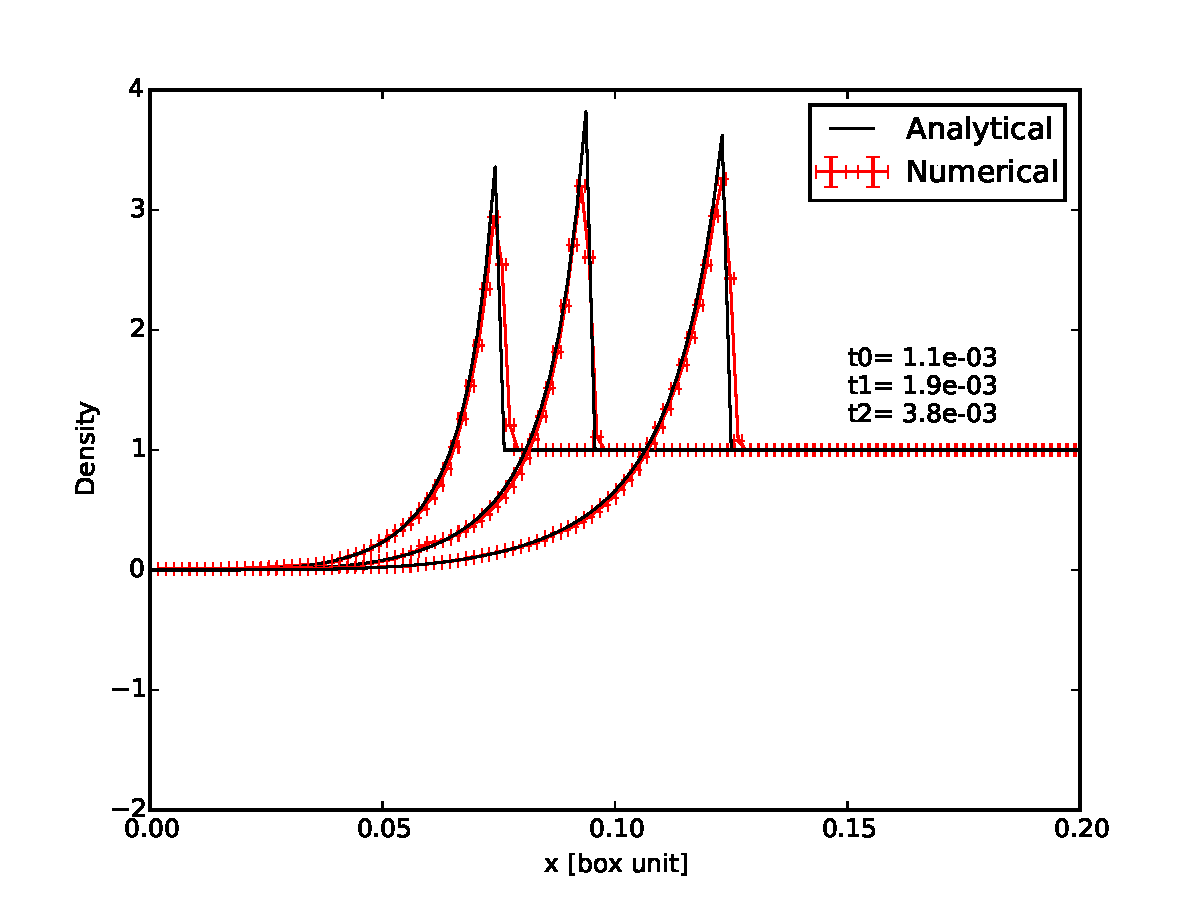
\includegraphics[width=.95\linewidth]{img/03/sedov/sedov_evol_8_den_lin.pdf} 
		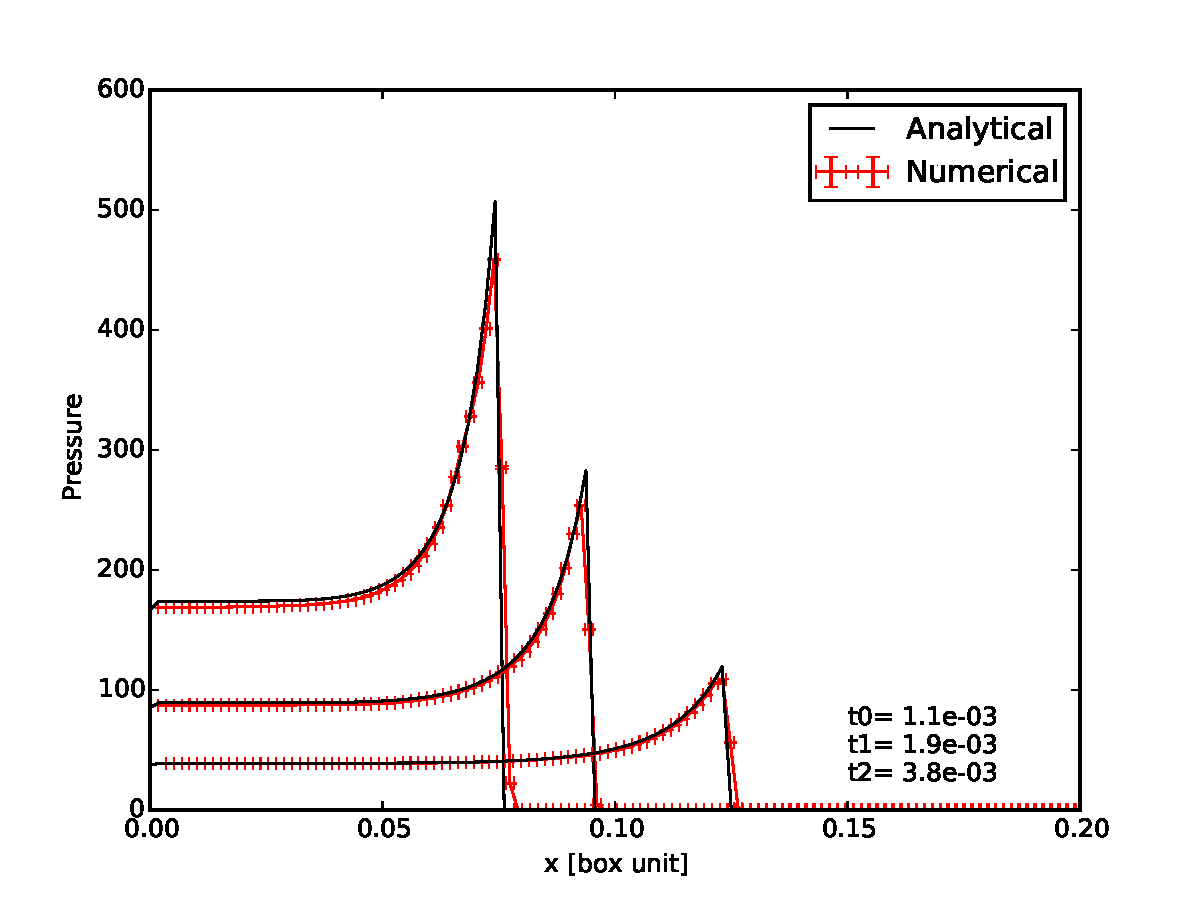
\includegraphics[width=.95\linewidth]{img/03/sedov/sedov_evol_8_pres.pdf} 
		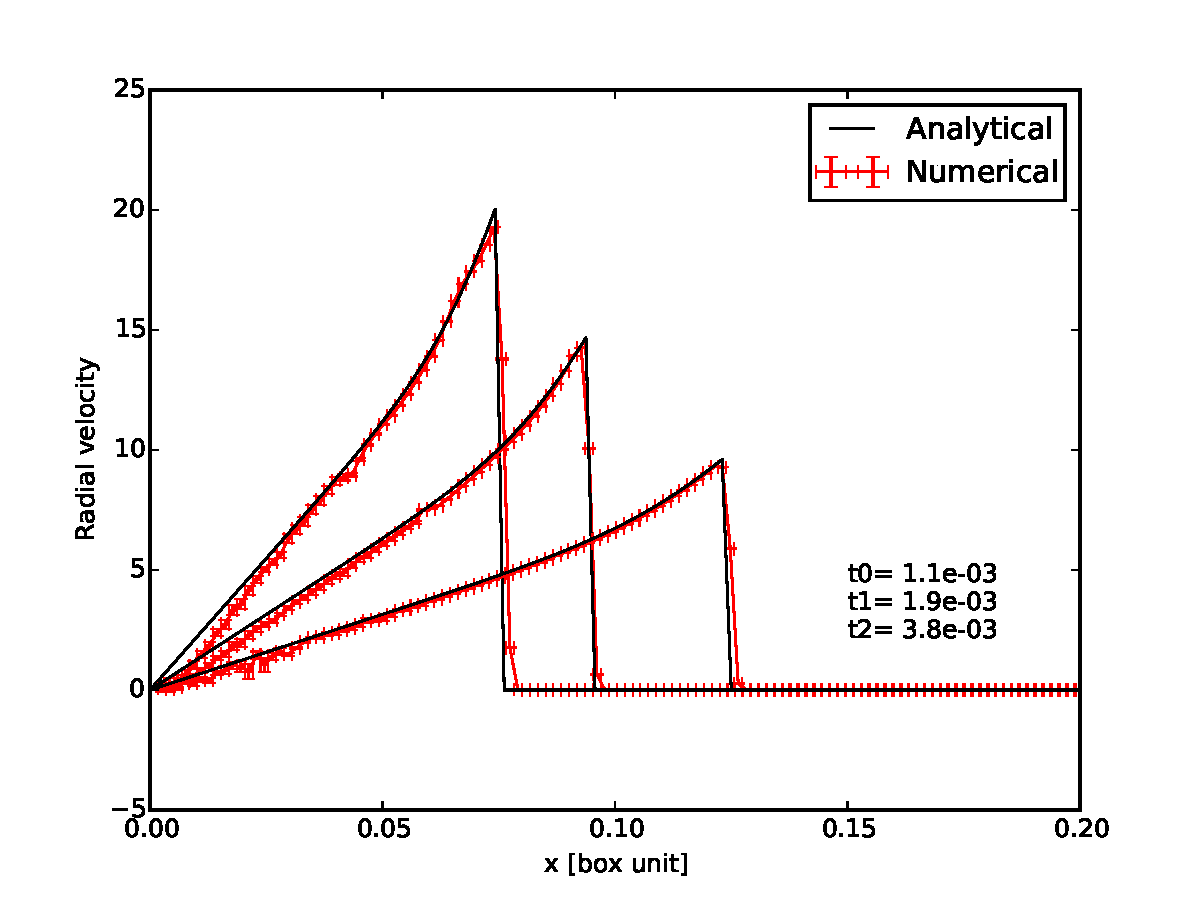
\includegraphics[width=.95\linewidth]{img/03/sedov/sedov_evol_8_vel.pdf} 
        \caption{Test de Sedov, evolution des differentes variables d'etats}
 		\label{fig:}
\end{figure}


\subsubsection{Sedov comparaison}

test en 128**3 avec raffinement, 3 niveaux

mise en place du raffinement :
raffinement sur le gradient 


\begin{figure}[bth]
        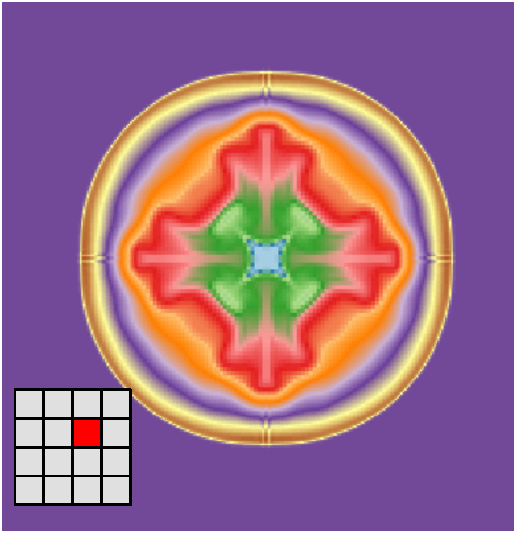
\includegraphics[width=.95\linewidth]{img/03/sedov/slice_therm1.pdf} 
		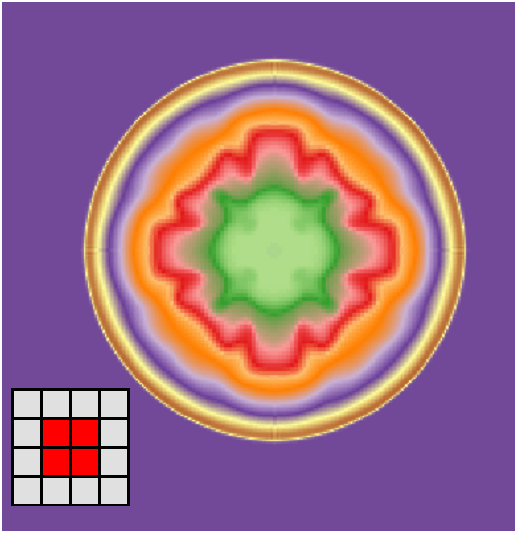
\includegraphics[width=.95\linewidth]{img/03/sedov/slice_therm4.pdf} 
		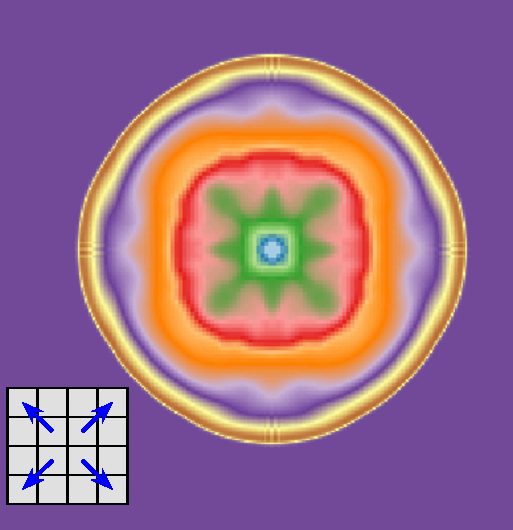
\includegraphics[width=.95\linewidth]{img/03/sedov/slice_kin.pdf} 
        \caption{Test de Sedov}
 		\label{fig:}
\end{figure}

\begin{figure}[bth]
        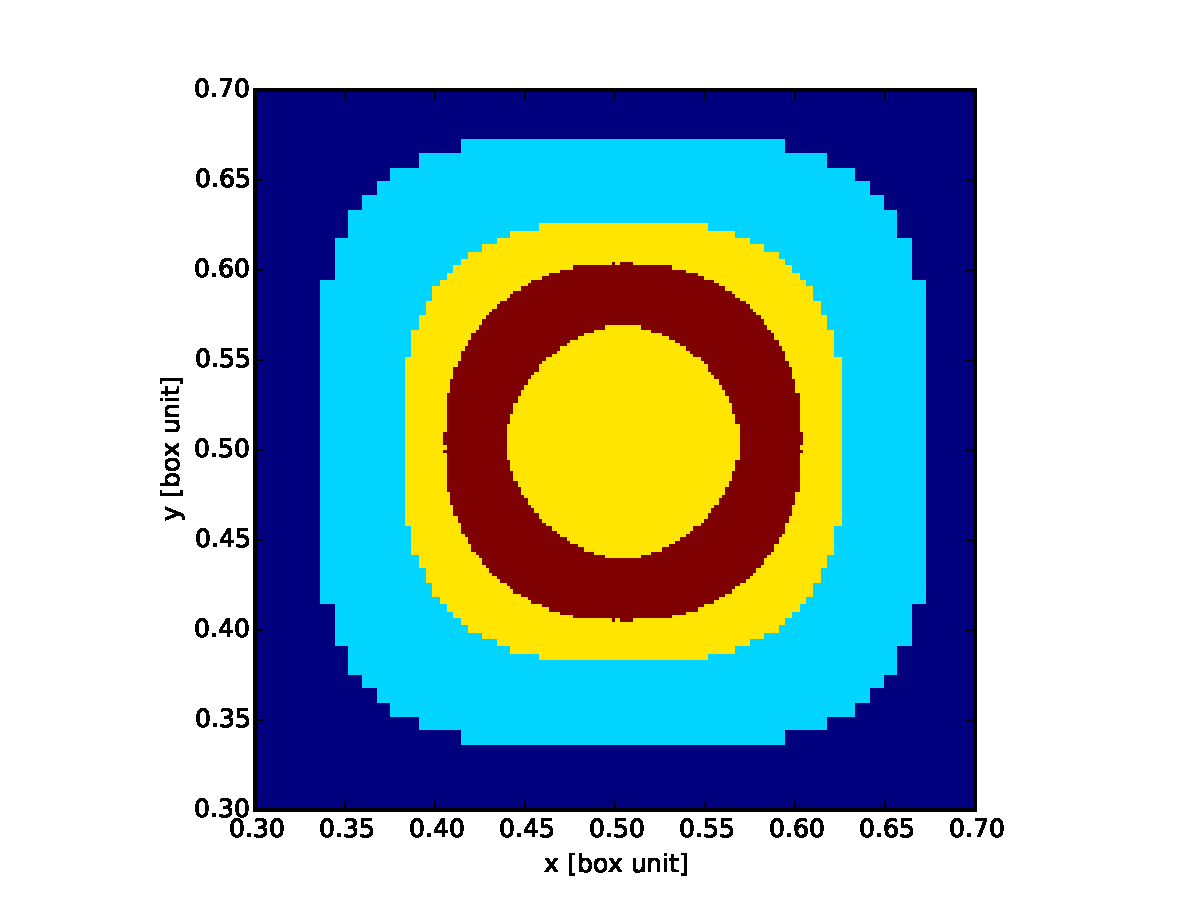
\includegraphics[width=.95\linewidth]{img/03/sedov/slice_th_1raf.pdf} 
        \caption{Test de Sedov, raffinement (mettre la color map) }
 		\label{fig:}
\end{figure}

\begin{figure}[bth]
        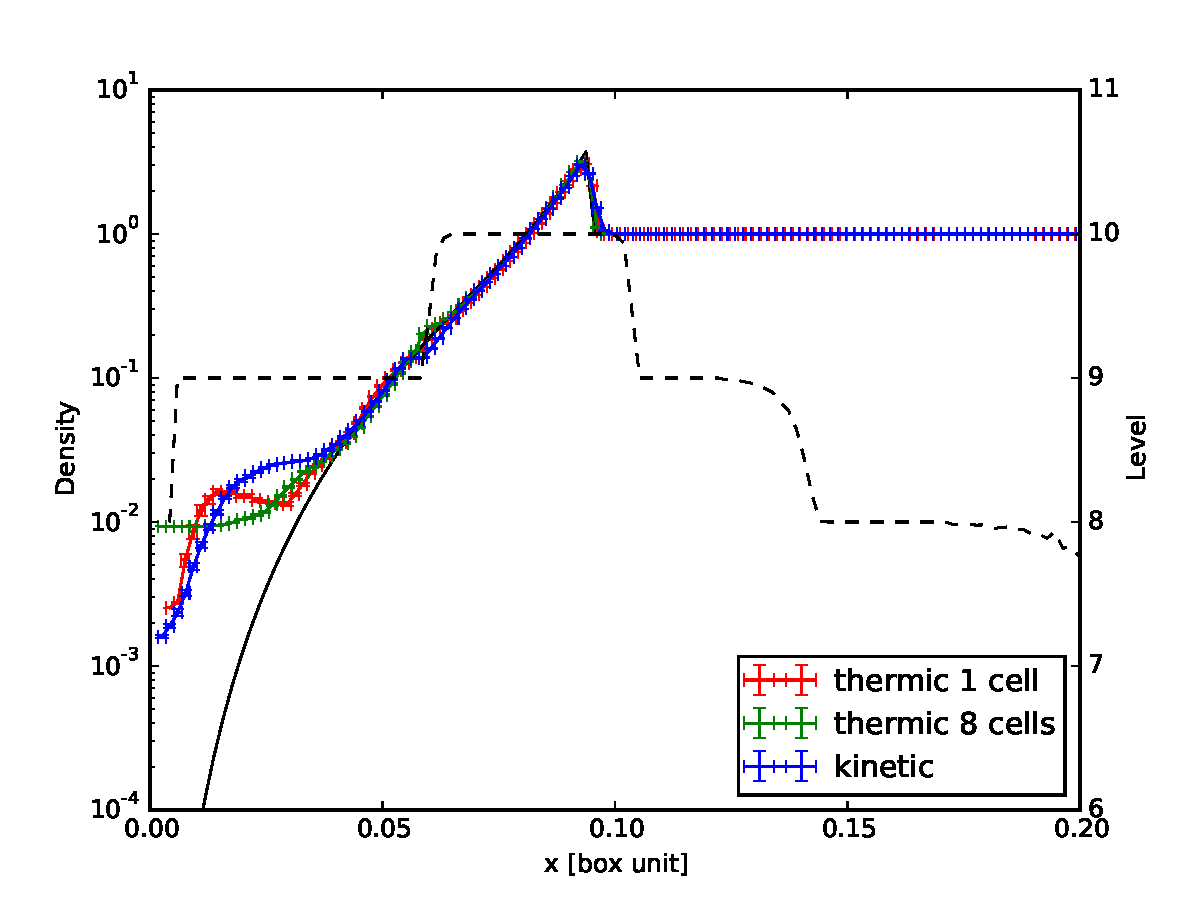
\includegraphics[width=.95\linewidth]{img/03/sedov/sedov_comp_profile_den.pdf} 
		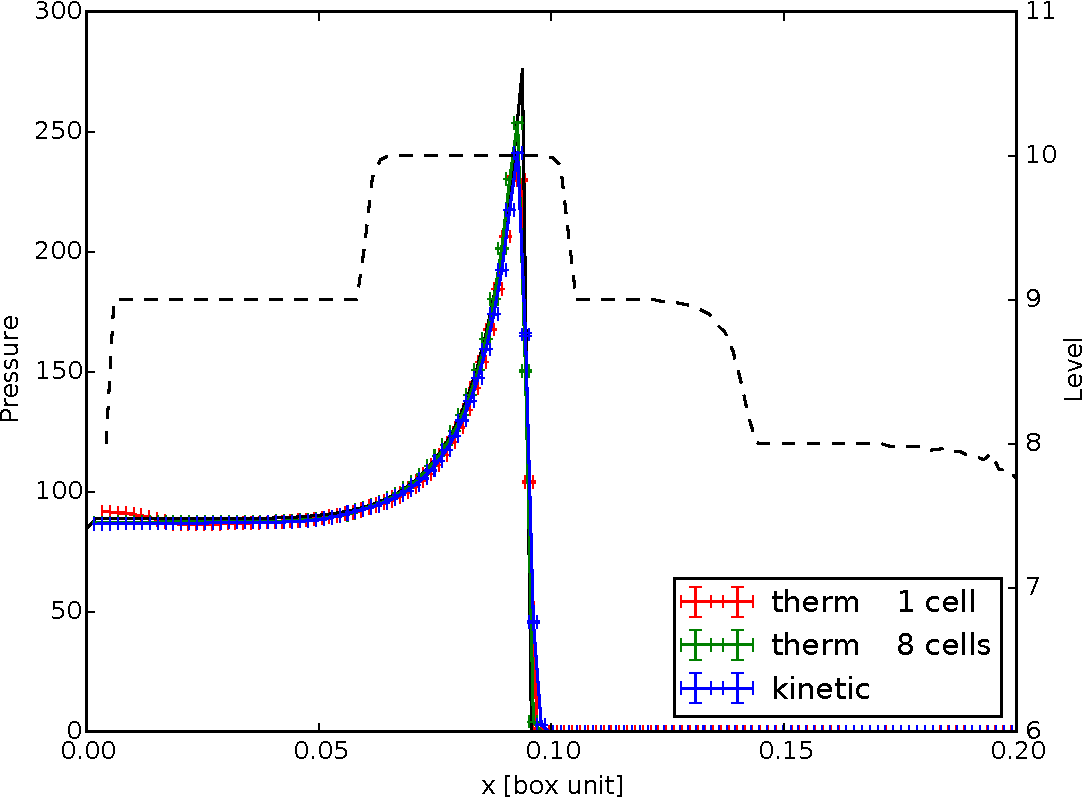
\includegraphics[width=.95\linewidth]{img/03/sedov/sedov_comp_profile_pres.pdf} 
		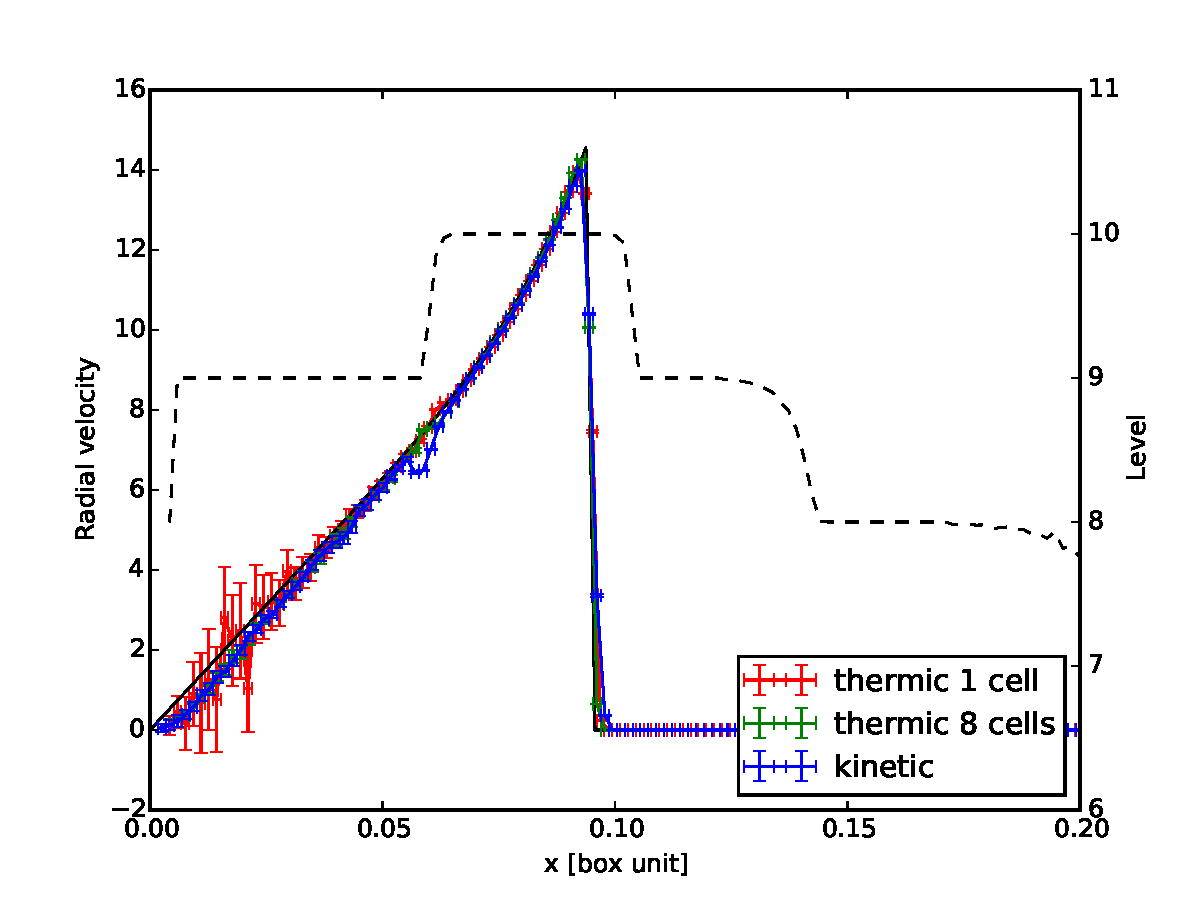
\includegraphics[width=.95\linewidth]{img/03/sedov/sedov_comp_profile_vel.pdf} 
        \caption{Test de Sedov, evolution des differentes variables d'etats}
 		\label{fig:}
\end{figure}




\subsection{Mes Implémentations}

\begin{equation}
e_{SN} = E_{SN}/8
\end{equation}

Then this energy is used to change the gas velocity by using:
\begin{equation}
    \Delta \overrightarrow{v_{gas}} = \sqrt{\frac{2e_{SN}}{\rho_g.dV}} \overrightarrow{u}
    \label{eq_sn_direct}
\end{equation}

le pas de temps\\
\section{test}
fonction de luminosité 
